\chapter{Iunctura}\label{ch:03}

\begin{chapter_outline}

  In this chapter, we demonstrate the benefits of mixing together distinct classes of models. In particular, we study the complementary between variational autoencoders (VAEs) and denoising diffusion probabilistic models (DDPMs). VAEs offer scalable amortised posterior inference and fast sampling but are also more and more outperformed by competing models such as normalizing flows (NFs) or deep-energy models. We improve VAEs by modelling the prior distribution of the latent variables with a diffusion process. The diffusion prior model improves upon Gaussian priors of classical VAEs and is competitive with NF-based priors.
  This contribution shows that connecting different classes of models can unlock modelling capacities and properties that are unreachable by each model class independently.
\end{chapter_outline}
\section{Prologue}
In this chapter, we argue that different (deep) probabilistic models shall not be studied independently. Building a broad and deep understanding of many probabilistic modelling frameworks unlocks many model combinations. These combinations may help reduce the weaknesses of each class of models separately while maintaining the assets of each class.

The gradient-descent-based training framework of neural networks is critical in developing these `super` deep probabilistic models that combine more than one type of model. This framework allows learning all components of a `super` model jointly as soon as the objective function is a differentiable function of the model's components. This chapter uses this feature to combine denoising diffusion probabilistic models and variational autoencoders.

As will see in the paper, combining DDPMs and VAEs is pretty straightforward and leads to better modelling for image synthesis. We believe that fostering further the interplay between different probabilistic models is essential in the development of the probabilistic modelling toolbox. In an ideal world, combining two classes of deep probabilistic models should be as simple as replacing a Normal distribution with a Laplace distribution in a probabilistic program. Building this ideal world should eventually help practitioners to define models with all the key properties required for their final application. The paper shall highlight the relevance of this idea.

\section{The paper: Diffusion Priors In Variational Autoencoders}

\subsection{Author contributions}
Gilles Louppe and I co-authored the paper. As the leading author, I developed the connections between diffusion models and variational autoencoders, did experiments, and wrote the article. In particular, I derived the ELBO associated with the denoising diffusion priors in VAES. Gilles Louppe supervised me throughout this project, offered suggestions, and helped write the paper.

\subsection{Reading tips}
The reader may skip section 2, which presents VAEs and DDPMs already introduced in the background chapter. The reader interested in deeply understanding the implementation of DDPMs should look at \citet{ho_denoising_2020}. The rest of the paper should flow naturally.

\subsection{Minor corrections}
There is a missing negative sign in Equation~(20) which becomes
$$\mathcal{L}(\mathbf{x}; \phi, \theta, \psi) := -\mathbb{E}_{q_{\psi}}\left[\log \frac{p_{\mathbf{\theta}}(\mathbf{x}|\mathbf{z})}{q_{\psi}(\mathbf{z}|\mathbf{x})} \right] + \mathbb{E}_{q_{\psi}}\left[ L_{\text{DDPM}}(\mathbf{z}_0; \phi)\right].$$

\includepdf[pages=-]{papers/innf_latent_diffusion.pdf}

\section{Epilogue}
\subsection{Behind the scenes}

Our initial motivation for combining diffusion models and VAEs was not to improve VAEs. Instead, we wanted to enable new types of noise for training diffusion models. Intuitively, the noise model is part of the inductive bias of the DDPM learning algorithm. Adapting the noise to the data modality might thus help to learn better models. In particular, we thought heat equations would provide an appealing inductive bias for image synthesis. Heat equation blurs the image along time; it corresponds to first discarding information about the details of the image and removing the semantic content only later in the noising process.

Our idea was to use a VAE formulation to bypass the closed-form gaussian kernel required for obtaining a tractable training objective. In addition, we thought playing with different diffusion speeds inside the latent variables of the VAE would eventually enforce different levels of structure between latent variables with varying schedules of diffusion. This would have provided an elegant way of extracting high and low-level semantic information from images.

Unfortunately, I did not figure out a good training algorithm for these models. Recently, \citet{rissanen2022generative} had a similar idea and achieved state-of-the-art image synthesis with a diffusion model based on the heat equation instead of the diffusion equation. Combining heat diffusion with VAEs to compress data into human-interpretable latent variables representing high and low-level features might be an interesting future research direction.

\subsection{Scientific impact}

According to Google Scholar, our article has received five citations between its publication in June 2021 and July 2022. It is interesting to contrast this number with the 48 citations received by \citet{vahdat2021score}, which was published in December 2021 at NeurIPS 2021 and was first released as a preprint on arXiv in June 2021. Although the ideas expressed in the two papers are similar, our work did not gain as much visibility as theirs. We acknowledge at least three \textbf{fair} reasons to explain this. First, publishing at NeurIPS brings much more visibility than at a workshop at ICML. This is natural as the reviewing process of NeurIPS is much stronger. Second, \citet{vahdat2021score} achieve state-of-the-art image synthesis by combining their idea with the proper neural architectures, training tricks and computation power.
In contrast to theirs, our work is more preliminary as it does not achieve state-of-the-art performance. Finally, advertising science is arguably nowadays as important as the science itself in machine learning.\citet{vahdat2021score} made an excellent job, as can be seen by one tweet from the first author who advertised their paper in \Cref{fig:cont_tweet} and had $6\times$ higher reach than a similar advertisement by Gilles Louppe in \Cref{fig:discrete_tweet}.

\subsection{Conclusion and opportunities}
Since the publication of this article, diffusion models have become very popular, owing part of their success to the astonishing results achieved by large text-to-images models created by OpenAI~\citep[$\text{DALL}\cdot\text{E} 2$][]{ramesh2022hierarchical} and Google~\citep[Imagen][]{saharia2022photorealistic}. Diffusion models have also percolated in audio modelling \citep{kong2020diffwave}. And close to our work, \citet{yu2022latent} recently proposed to use energy-based models trained with denoising score matching to model the prior distribution of VAEs for interpretable text modelling.

In the near future, the attractivity of diffusion models for modelling distributions over images, and other data modalities, should stay high. There remain many open questions such as \textit{why do diffusion models represent high dimensional data such as images so well?} The answer relies upon the inductive bias of diffusion models; however, which part exactly is an open question. Diffusion models also have some limitations. The sampling procedure is convoluted as it requires evaluating the neural network modelling the denoising function (or score function) many successive times. Pushing further the connections between diffusion models and other probabilistic models such as normalizing flows and VAEs might help reduce the sample synthesis's complexity.

\begin{figure*}[h]
  \centering
  \begin{subfigure}[b]{.48\textwidth}
    \centering
    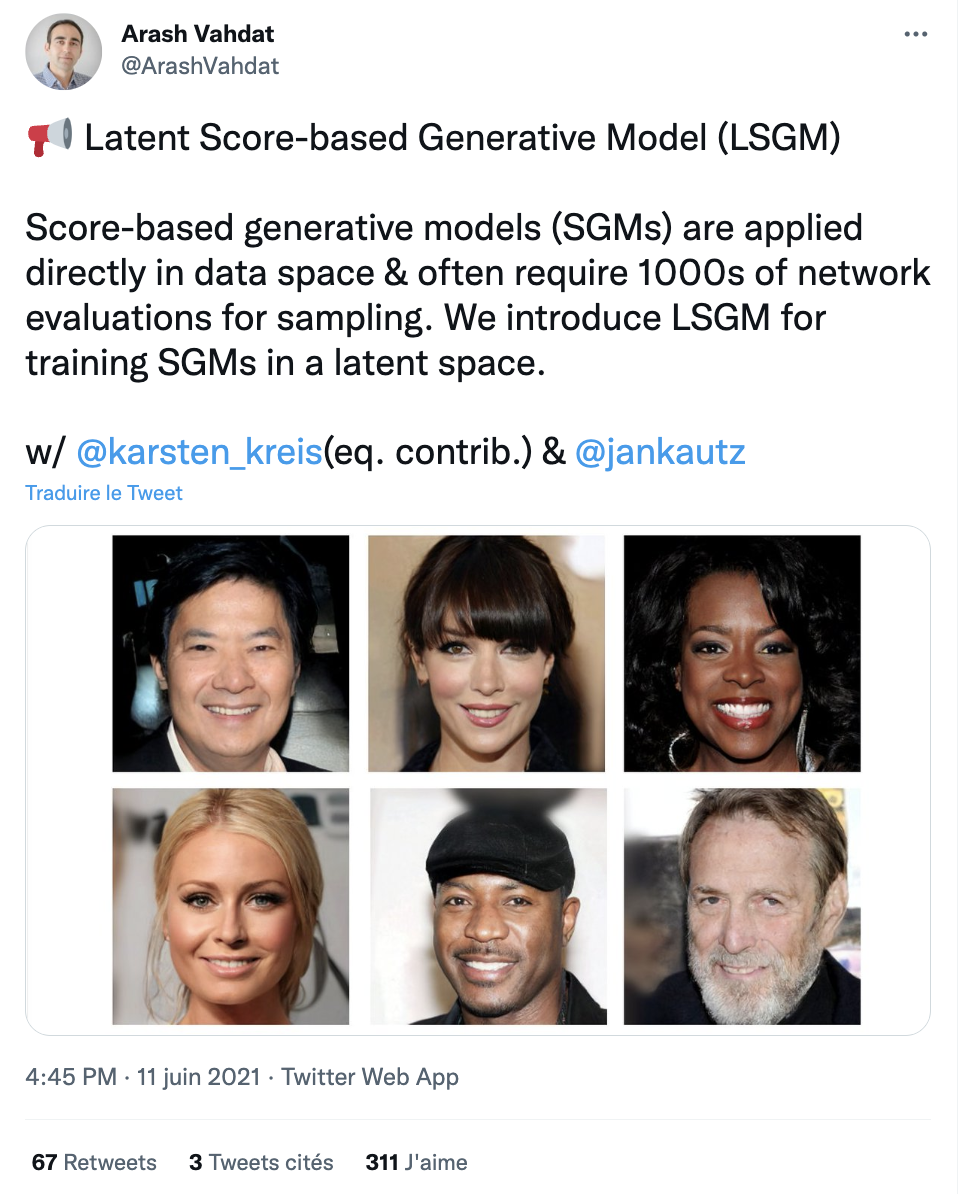
\includegraphics[width=.85\textwidth]{figures/impact_scholar/cont_diff_tweet.png}
    \caption{}
    \label{fig:cont_tweet}
  \end{subfigure}
  \begin{subfigure}[b]{.48\textwidth}
    \centering
    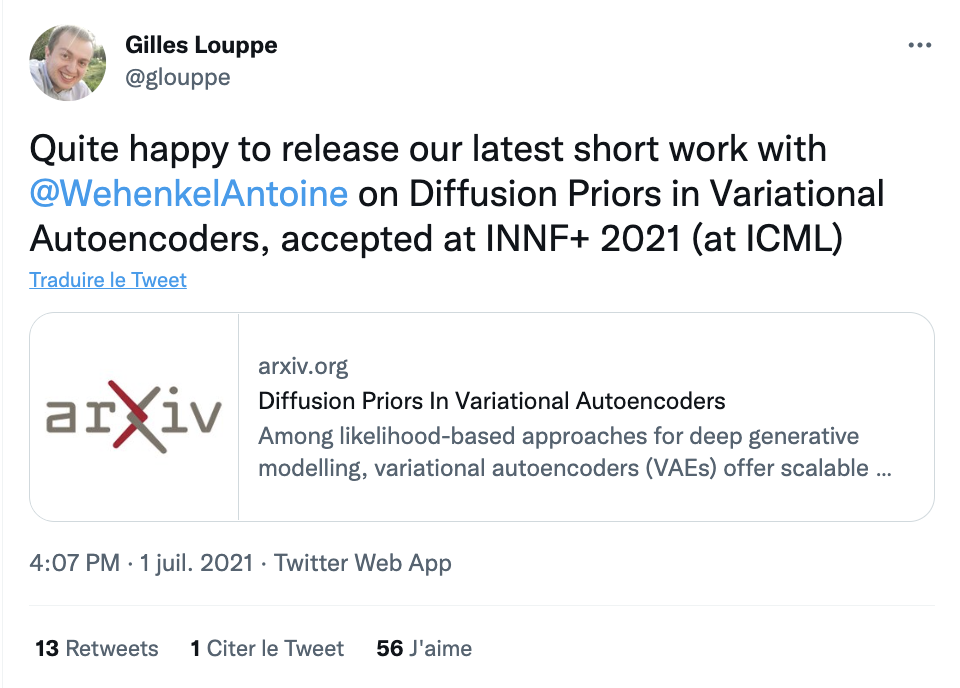
\includegraphics[width=.9\textwidth]{figures/impact_scholar/discret_diff_tweet.png}
    \caption{}
    \label{fig:discrete_tweet}
  \end{subfigure}
  \caption{Tweets advertising (\textbf{a}) continuous-time diffusion models in the latent space from \citet{vahdat2021score} (\textbf{b}) discrete-time diffusion models in the latent space.}
\end{figure*}
